\section{Machine Learning}

Consideremos un conjunto de datos $X = (x_1, \dots , x_N)$ donde para cada $i \in {1, \dots, N}$, $x_i = [x_{i}^1 , \dots, x_{i}^M]$ es decir, un conjunto de $N$ datos con $M$ features cada uno. Consideremos además $Y = (y_1, \dots , y_N)$ las etiquetas o labels cada cada dato. En problemas de clasificación binario, $y_i \in \{ 0, 1\}$ y en problemas de clasificación multiclase, $y_i \in \{1, \dots L\}$.

\subsection{Decision Trees}

Un árbol de decisión es un modelo de aprendizaje \textbf{supervisado} utilizado para problemas de \textbf{regresión} y \textbf{clasificación}. El objetivo es aprender simples reglas de decisión a partir de las features. 

\begin{figure}[H]
    \center
    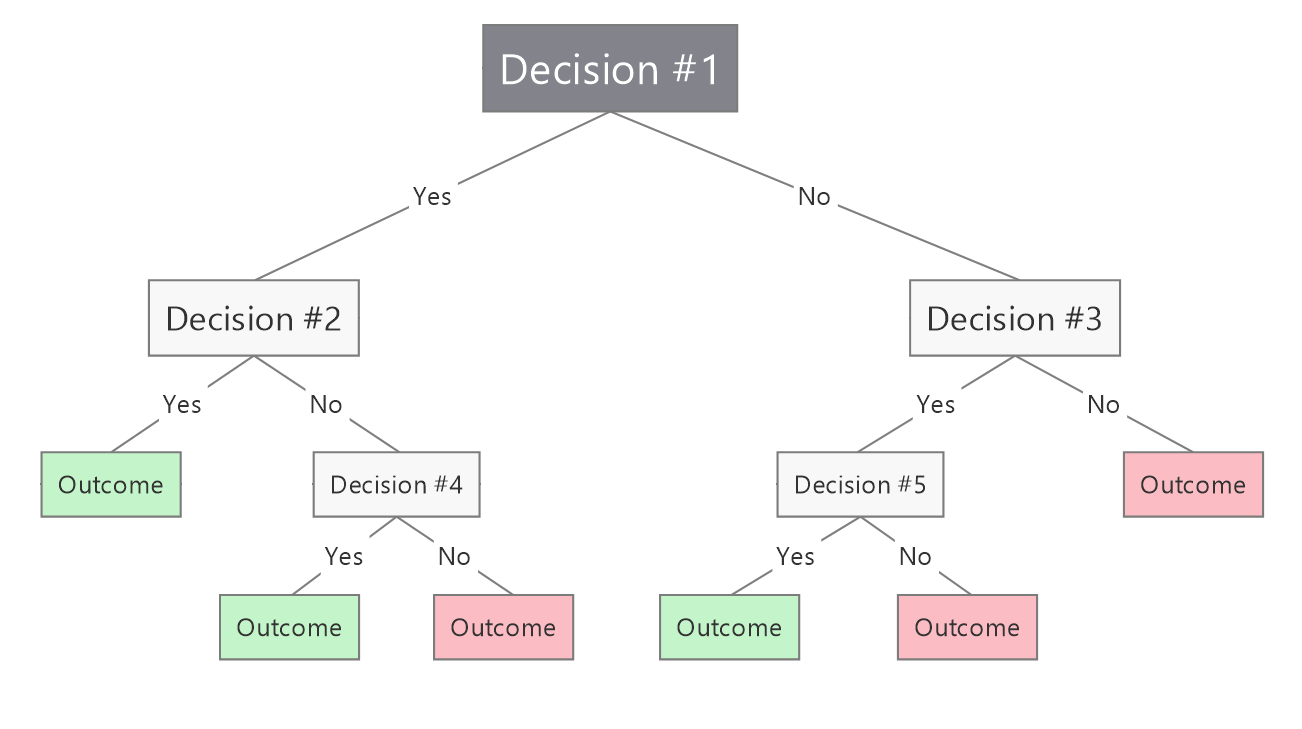
\includegraphics[scale=0.25]{notebooks/ML/img/decision_tree_diagram.png}
    \caption{Decision Tree Diagram}
\end{figure}

En el caso de un problema de clasificación, la variable a escoger y el corte correspondiente se puede elegir como aquel que minimice el desorden de los elementos. Definimos primero la \textbf{entropía} según 
$$H(p) = - \sum_{j=1}^{L}p_j\log_{2}p_j$$

donde $p_j$ es la frecuencia relativa del label $j$ en un grupo. Notar que la entropía es mínima cuando el grupo solo tiene elementos de la clase 0 o de la clase 1 ($p_j = 1$) y máxima cuando hay la misma cantidad de elementos de cada clase ($p_j = \frac{1}{2}$). 

\begin{figure}[H]
    \center
    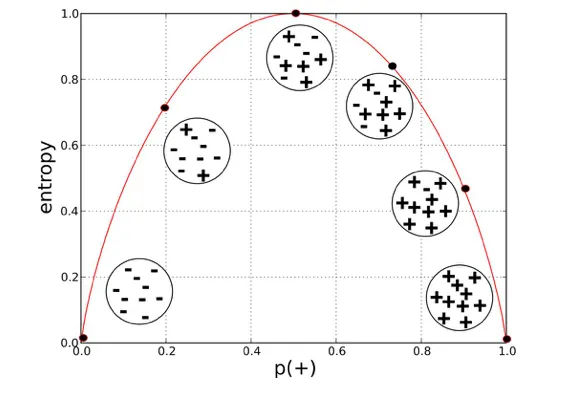
\includegraphics[scale=0.3]{notebooks/ML/img/entropy_diagram.png}
    \caption{Entropy Diagram}
\end{figure}

Con la entropía ya definida, definamos la \textbf{Information Gain} como 
$$IG(S,D) = H(S) - \sum_{V \in D}\frac{|V|}{|D|}H(V)$$

Donde el primer término es la entropía antes del split y el segundo término es la suma de las entropías después del split. Podemos iterar hasta que la Information Gain no tenga modificaciones (es decir, llegar a los nodos puros) pero esto podría traer problemas de \textit{overfitting}, en general esto se regula con la profundidad del árbol y escogiendo en cada iteración, la división que maximiza el IG. 

\begin{figure}[H]
\begin{subfigure}{.5\textwidth}
    \center
    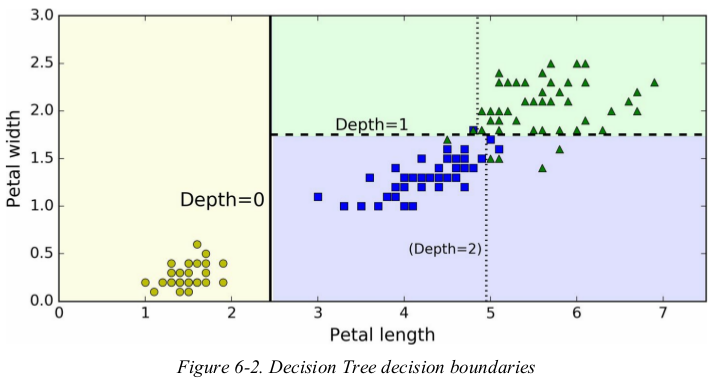
\includegraphics[scale=0.3]{notebooks/ML/img/decision_tree_data.png}
    \caption{Decision Tree Boundaries}
\end{subfigure}%
\begin{subfigure}{.5\textwidth}
    \center
    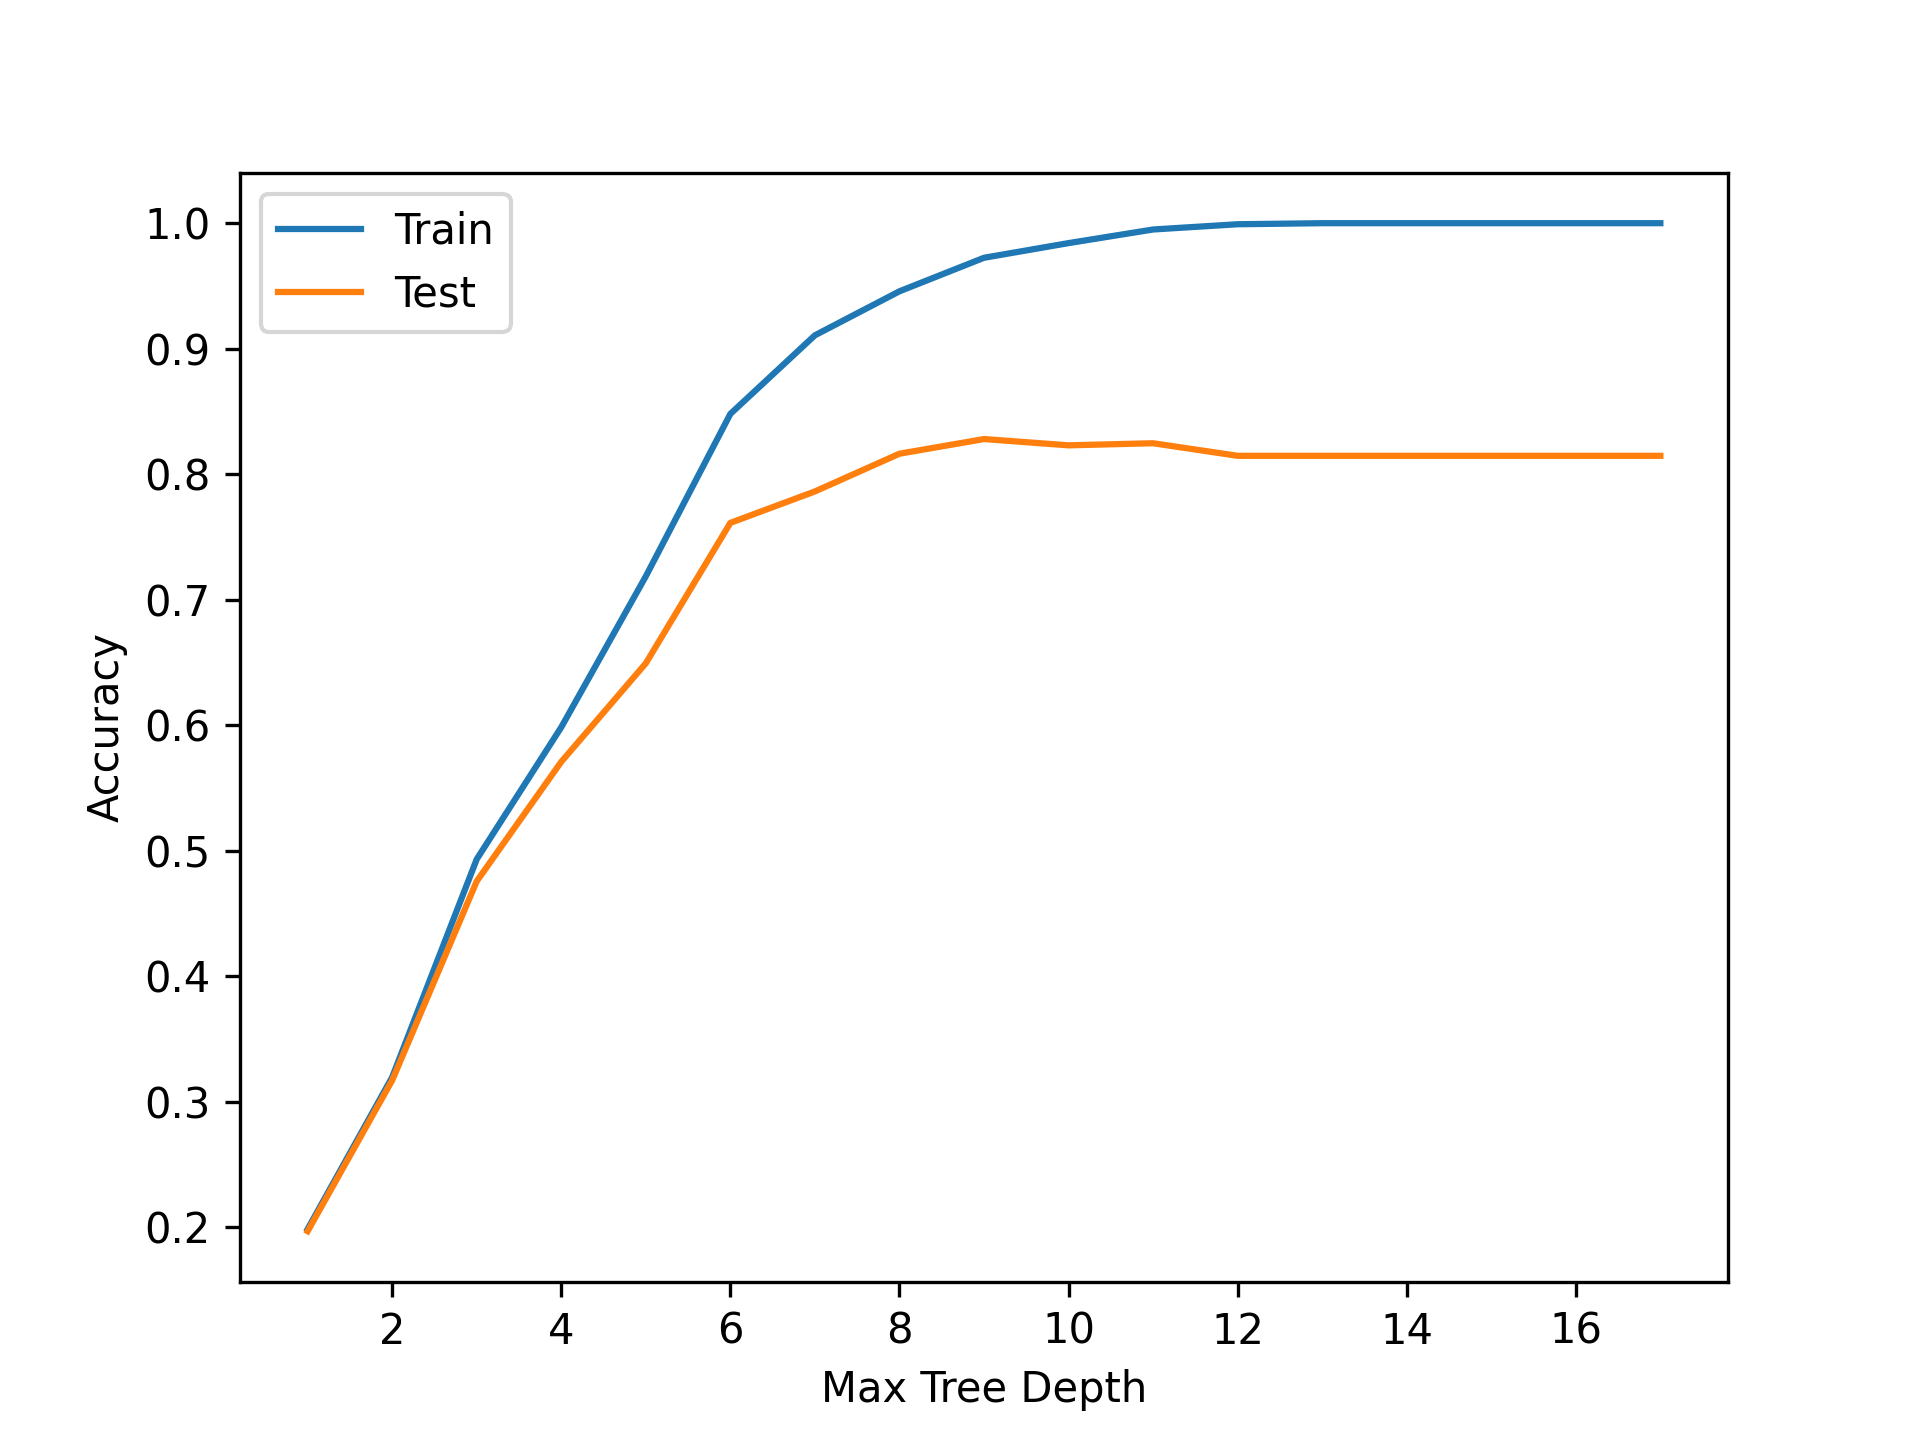
\includegraphics[scale=0.4]{notebooks/ML/img/max_depth_decision_tree.png}
    \caption{Max Depth and Accuracy}
\end{subfigure}
\caption{Decision Tree Implementation}
\label{fig:fig}
\end{figure}

En vez de la entropía, es posible usar otro indicador como el \textbf{Gini Index} definido como: 
$$G(p) = 1 - \sum_{j=1}^L p_j^2$$

\subsection{Random Forest}

\subsubsection{Ensemble Methods}

Los \textbf{métodos de ensamblaje} son aquellos en los que se combinan múltiples estimadores entrenados sobre los datos para generar una predicción más robusta (menor varianza) y generalizada. La predicción final se puede realizar por \textit{Majority Voting}, \textit{Simple Average} o \textit{Weighted Average}.

Existen 3 estrategias principales en los métodos de ensamblaje: 
\begin{enumerate}
    \item \textbf{Bagging}: Corresponde a una abreviación de \textit{Bootstrap Aggregating}, esta estrategia entrena cada estimador base con una \textbf{muestra con reemplazo} de ejemplos del conjunto de entrenamiento. 
    \item \textbf{Boosting}: Esta estrategia se basa en entrenar secuencialmente estimadores base débiles que \textbf{aprenden de los errores del anterior} para crear un estimador robusto.
    \item \textbf{Stacking}: Este método combina las predicciones de múltiples estimadores fuertes en una sola. 
\end{enumerate}

\begin{figure}[H]
    \center
    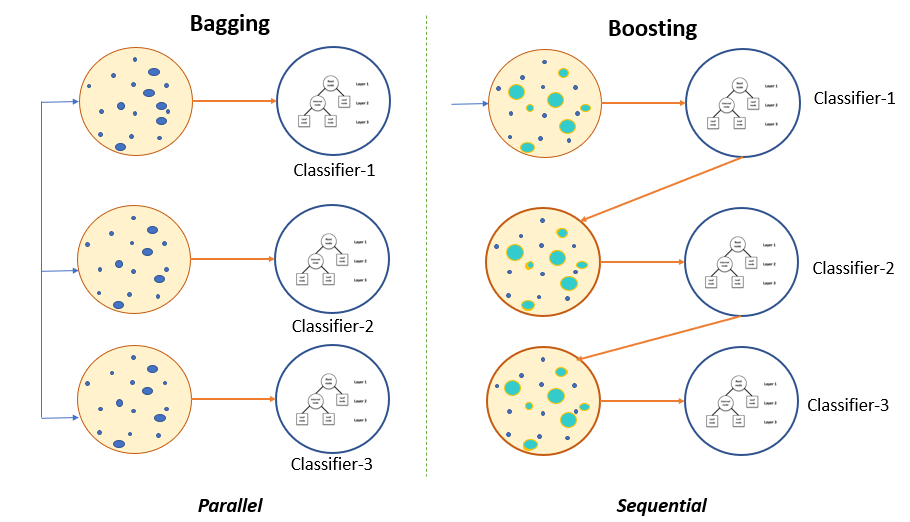
\includegraphics[scale=0.25]{notebooks/ML/img/bagging_and_boosting_diagram.png}
    \caption{Bagging and Boosting Diagram}
\end{figure}


El algoritmo de \textit{Random Forest} es un método \textbf{supervisado de ensamblaje} basado en \textit{Decision Trees}. Este, utiliza la estrategia de \textbf{bagging} para entrenar cada árbol de decisión sobre muestras con reemplazo del conjunto de entrenamiento y además, cada árbol es entrenado sobre un \textbf{subconjunto aleatorio de features} para asegurar que no haya similitud entre ellos. Ambas estrategias permiten mejorar la precisión del modelo y controlar el  \textit{overfitting}.

\begin{figure}[H]
    \center
    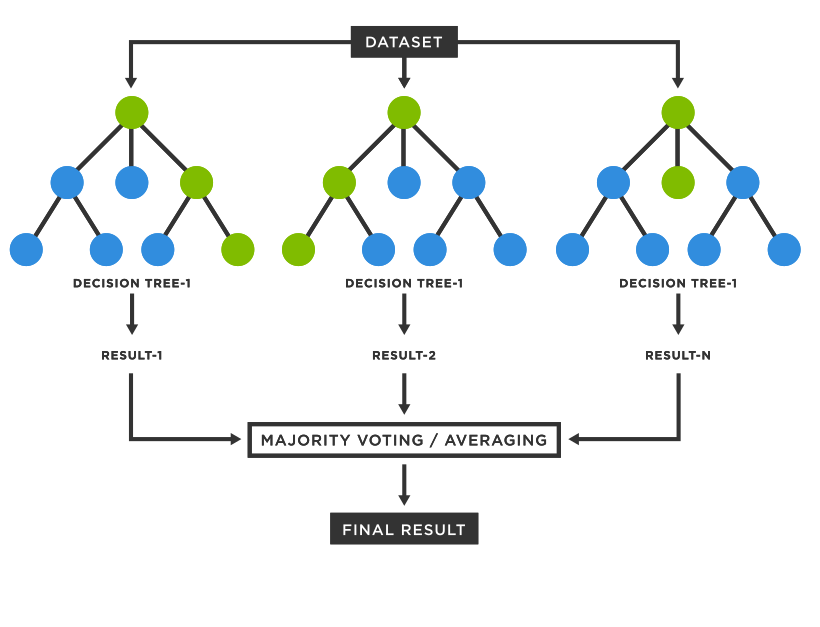
\includegraphics[scale=0.25]{notebooks/ML/img/random_forest_diagram.png}
    \caption{Random Forest Diagram}
\end{figure}

\subsection{Support Vector Machines}

